\chapter{Implementation: LSP server architecture}
\label{lspimplementation}

The following chapters will discuss how CCDetect-LSP is implemented, and especially
focuses on our novel algorithm based on dynamic extended suffix arrays. The current
chapter will look at the LSP integration and how source code is initially indexed, while
the following two chapters will discuss first how clones are initially detected and then
how this analysis in incrementally updated as source code changes.

CCDetect-LSP is integrated into IDEs via LSP. The tool starts up as an LSP server, which
an IDE client can connect to and send/receive messages from. The goal of the LSP
client-server interaction is to give users of the tool an overview of all clones as they
appear in source code, and allow them to navigate between matching clones. CCDetect-LSP is
implemented in Java with the LSP4J library which provides an abstraction layer on top of
the protocol which is easier to work with programmatically.

\begin{figure}[t]
	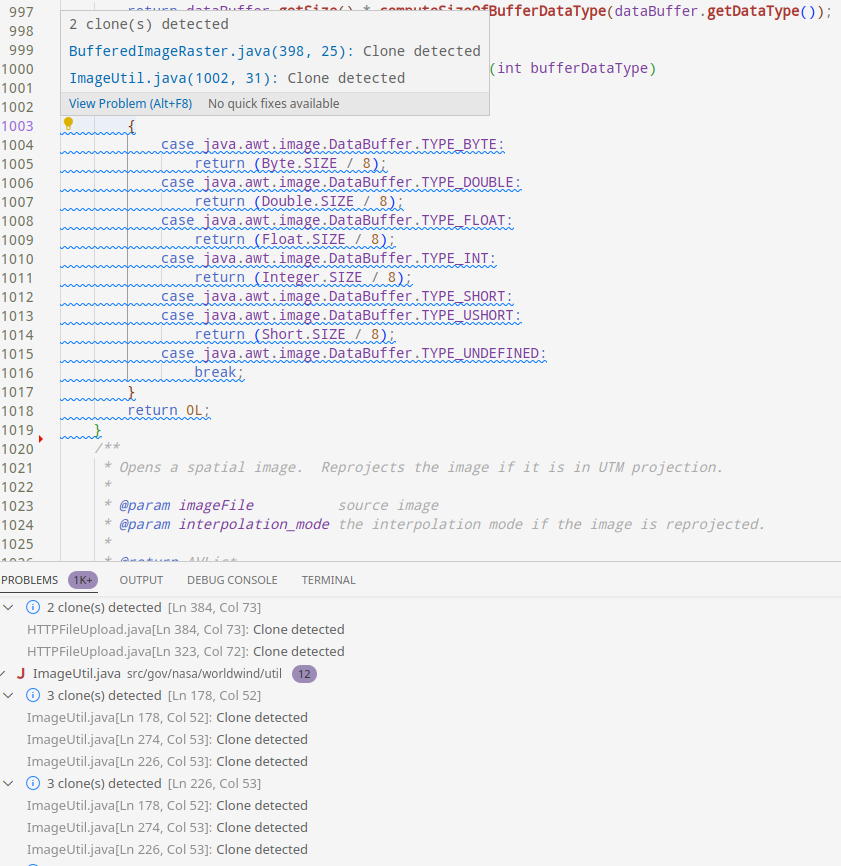
\includegraphics[width=\textwidth]{figures/vscodecodeclone.png}
	\caption{Code clones displayed in the VSCode IDE}
	\label{fig:vscodeclones}
\end{figure}

Figure \ref{fig:vscodeclones} shows how clones are displayed in the VSCode IDE. The image
shows a section of a file where a Java switch statement has been duplicated in two other
files. Code clones are displayed inline in the file as an ``Information'' diagnostic, and
when hovered over, the client shows the \verb|DiagnosticRelatedInformation| information of
the diagnostic where all the matching clones are displayed and can be clicked to navigate
to the corresponding match. For a client which may not implement the
\verb|DiagnosticRelatedInformation| message\footnote{Added to LSP in version 3.16,
released in 2020. In our experience, some IDEs do not implement this feature.}, invoking a
code-action to navigate to the matching clone is another option.

The following user-stories shows how interaction with the LSP server works.

\begin{itemize} 

    \item A programmer wants to see code clones for a file in their project, the
        programmer opens the file in their IDE and is shown diagnostics inline with the
        code wherever there are detected clones. The matching code clones are not
        necessarily in the same file.

	\item A programmer wants to see all code clones for the current project. The
	      programmer opens the IDEs diagnostic view and will see all code clones detected
	      as diagnostics there. The diagnostic will contain information like where the clone
	      exists, and where the matching clone(s) are.

    \item A programmer wants to jump to one of the matches of a code clone in their IDE.
        The programmer moves their cursor to the diagnostic and will see a list of the
        matching code clones. The programmer selects any of the code clones which will
        open the file and location of the selected code clone. Alternatively, a
        code-action can be invoked to navigate, if the client does not implement the
        \verb|DiagnosticRelatedInformation| interface.

      \item A programmer wants to refactor a set of clones by applying the
          ``extract-method'' refactoring (not implemented by CCDetect-LSP). The programmer
          performs the necessary refactorings, and will see that the refactored clones are
          no longer detected when the LSP server incrementally updates its analysis.

\end{itemize}

\begin{figure}
	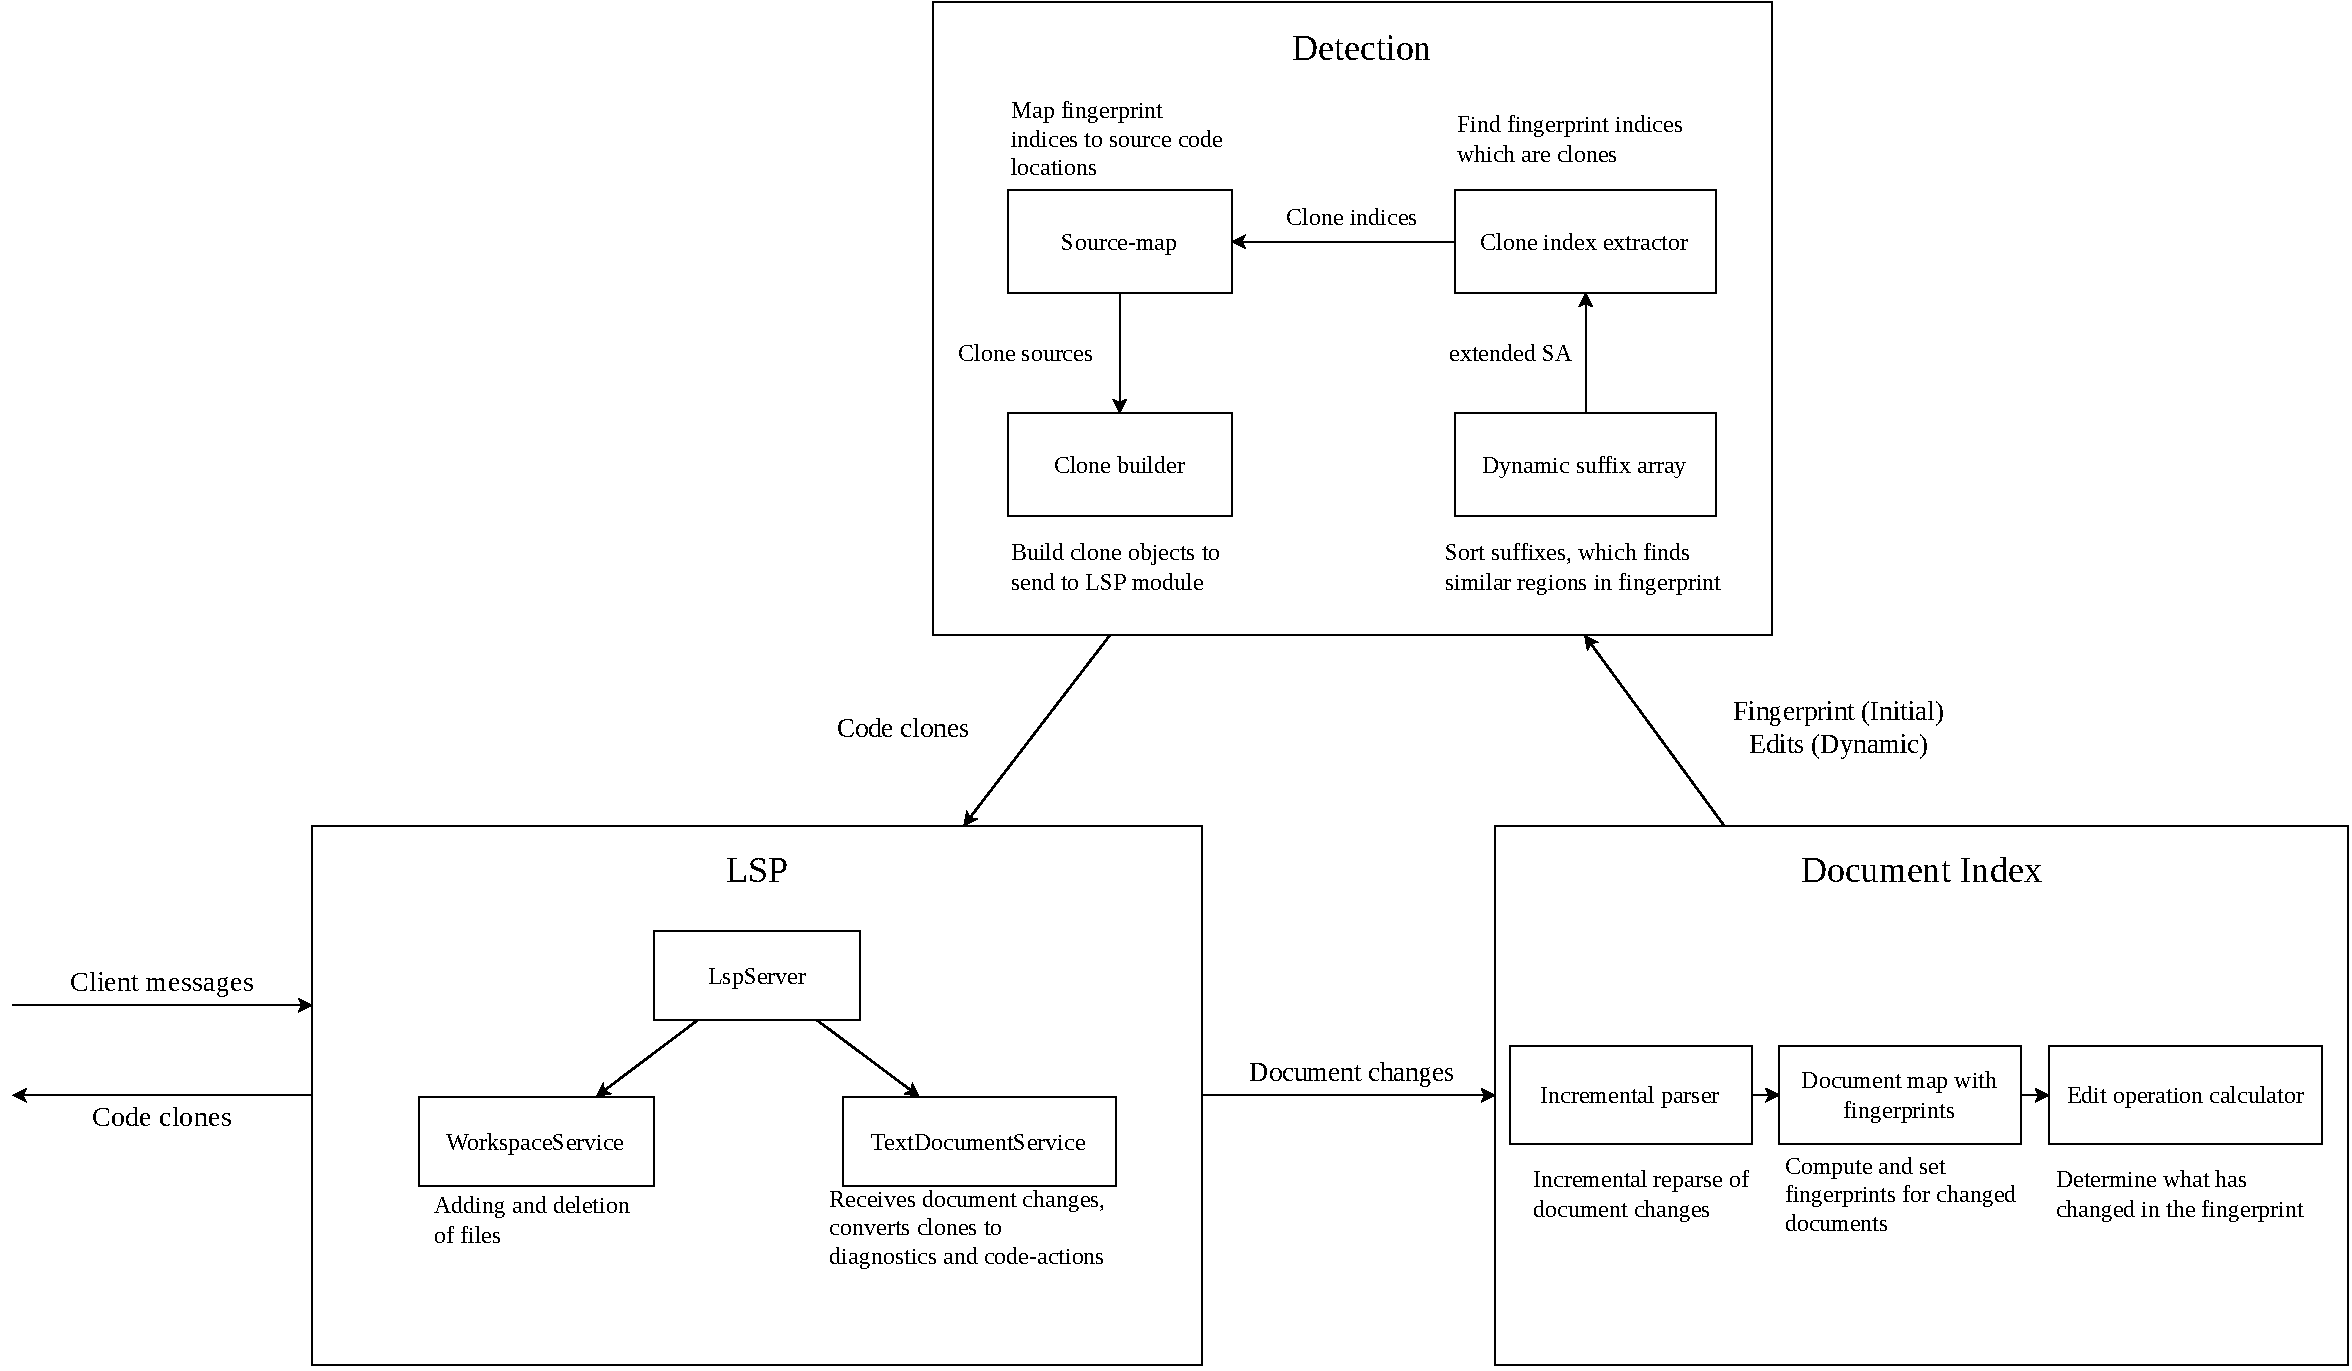
\includegraphics[width=\textwidth]{figures/architecture.drawio.pdf}
	\caption{Tool architecture}
	\label{fig:architecture}
\end{figure}

Figure \ref{fig:architecture} shows the architecture of the tool. The LSP module
communicates with the IDE and delegates the work of handling documents to the document
index. Detection of clones is delegated to the detection module. The LSP module receives a
list of clones from the detection module which is then converted to LSP diagnostics and
code-actions which is finally sent to the client.

\section{Document index}

Upon starting, the LSP server needs to index the project. This involves creating an index
and inserting all the relevant documents in the code base. A document contains the content
of a file along with extra information such as the file's URI and some information which
is useful for the later clone detection. We define the following record for our documents:

\begin{lstlisting}
    Document {
        String uri,
        String content,
        AST ast,

        // Location in fingerprint
        int start,
        int end

        // Used for incremental updates
        int[] fingerprint,
        boolean open,
        boolean changed,
    }
\end{lstlisting}

Each document in the index primarily consists of the contents, the URI and the AST of the
document in its current state. Storing the AST will be useful for the incremental
detection algorithm.

There are two things to consider when determining which files should be inserted into the
index. First, we are considering only files of a specific file type, since the tool does
not allow analysis of multiple programming languages at the same time. Therefore, the
index should contain for example only \verb|*.java| files if Java is the language to
analyze. Secondly, all files of that file type might not be relevant to consider in the
analysis. This could for example be generated code, which generally contains a lot of
duplication, but is not practical or necessary to consider as duplicate code, since this
is not code which the programmer interact with directly. Therefore, the default behavior
is to consider only files of the correct file type, which are checked into Git. The tool
supports adding all files in a folder, or all files checked into Git.

When a document is first indexed by the server, the file contents is read from the disk.
However, as soon as the programmer opens this file in their IDE, the source of truth for
the files content is no longer on the disk, as the programmer is changing the file
continuously before writing to the disk. The LSP protocol defines multiple JSON-RPC
messages which the client sends to the server in order for the server to keep track of
which files are opened, and the state of the content of opened files.

Upon opening a file, the client will send a \verb|textDocument/didOpen| message to the
server, which contains the URI for the opened file. The index will at this point set the
flag \verb|open| for the relevant document and stops reading its contents from disk.
Instead, updates to the file are obtained via the \verb|textDocument/didChange| message.
This message can provide either the entire content of the file each time the file changes,
or it can provide only the changes and the location of the change. Receiving only the
changes will be useful for this algorithm when the analysis incrementally reparses the
document.

\section{Displaying and interacting with clones}

When detection is finished and the list of clones is ready, the LSP module will convert
clones into diagnostics and code-actions which can be interacted with from the client. For
diagnostics, each clone object is converted into a diagnostic which has a range and some
information about the clone. The diagnostic displays an error in the client which also has
information for each matching clone. This is achieved this by attaching
\verb|DiagnosticRelatedInformation| to a diagnostic which is defined in the protocol. When
all the code clones have been converted to diagnostics, the server sends a
\verb|textDocument/publishDiagnostics| message which sends all the diagnostics to the
client in JSON-RPC format. For code-actions, the process is similar, for each clone pair,
we create a code-action which navigates from one to the other, using the
\verb|window/showDocument| message. These code-actions are similarly sent to the client
via the \verb|textDocument/codeAction| message, but this message is only invoked when the
client specifically requests code actions at a certain location.

